\documentclass[12pt, letterpaper, a4paper]{article}
\usepackage{graphicx}
\usepackage{textcomp}
\usepackage[hungarian]{babel}
\usepackage[T1]{fontenc}
\usepackage[utf8]{inputenc}
\usepackage{caption}
\usepackage{subcaption}
\usepackage{csquotes}
\graphicspath{{../Pictures/}}
\usepackage[
    style=ieee,
  ]{biblatex}
\addbibresource{soc.bib}

\usepackage{listings}
\usepackage[svgnames]{xcolor}
\usepackage{tikz}
\usetikzlibrary{shapes.geometric, arrows, calc}

\usepackage{float}

\definecolor{dkgreen}{rgb}{0,0.6,0}
\definecolor{gray}{rgb}{0.5,0.5,0.5}
\definecolor{mauve}{rgb}{0.58,0,0.82}

\lstset{frame=tb,
  language=Bash,
  aboveskip=3mm,
  belowskip=3mm,
  showstringspaces=false,
  columns=flexible,
  basicstyle={\small\ttfamily},
  numbers=none,
  numberstyle=\tiny\color{gray},
  keywordstyle=\color{blue},
  commentstyle=\color{dkgreen},
  stringstyle=\color{mauve},
  breaklines=true,
  breakatwhitespace=true,
  tabsize=2
}

\lstdefinestyle{cstyle}{
  language=C,
  basicstyle=\footnotesize\ttfamily,  % smaller fixed-width font
  keywordstyle=\color{RoyalBlue},     % keywords like for, if, while
  commentstyle=\color{DarkGreen}\itshape,  % italic green comments
  stringstyle=\color{orange!80!black},     % orange strings
  identifierstyle=\color{black},      % variable/function names
  numberstyle=\tiny\color{gray},
  numbers=left,
  numbersep=8pt,
  frame=none,
  showspaces=false,
  showstringspaces=false,
  showtabs=false,
  tabsize=2,
  captionpos=b,
  breaklines=true,
  breakatwhitespace=true,
  aboveskip=0.5em,
  belowskip=0.5em,
  lineskip=-1pt,
  morekeywords={uint8_t, memcpy, memset}, % highlight C stdlib/uint types
  morekeywords=[2]{compare,merge,sort,media_filter_scalar},
  keywordstyle=[2]\color{purple}
}

\lstdefinestyle{pythonstyle}{
  language=Python,
  basicstyle=\ttfamily\footnotesize,
  keywordstyle=\color{RoyalBlue}\bfseries,
  commentstyle=\color{DarkGreen}\itshape,
  stringstyle=\color{orange!80!black},
  numberstyle=\tiny\color{gray},
  numbers=left,
  numbersep=8pt,
  frame=none,
  showstringspaces=false,
  tabsize=4,
  breaklines=true,
  breakatwhitespace=true,
  captionpos=b,
}

\tikzstyle{box} = [rectangle, rounded corners, minimum width=3cm, minimum height=0.5cm,text centered, draw=black, fill=orange!30]
\tikzstyle{arrow} = [thick,->,>=stealth]


\title{\textcolor{RoyalBlue}{\textbf{Heterogén SoC rendszerek házi feladat}}}
\author{\textcolor{RoyalBlue}{Batcher Odd-Even-Merge algoritumus skalár megvalósítás} \\ \\ Nyiri Levente}
\date{2025 Október}
\begin{document}
\selectlanguage{hungarian}
\maketitle

\newpage

\section{Algoritmus}
Batcher Odd-Even-Merge algoritmusa először elfelezi a tömböt két részre, ezeket rendezi, külön összehasonlítja a páros elemeket a párosokkal, a páratlanokat a páratlanokkal, és végül a szomszédos elemeket egymással.

Ez egy rekurzív algoritmus. Két részből áll: egy olyan algoritmus ami a két rendezett felet kialakítja (sort), és egy olyan ami ezeket a rendezett feleket felhasználva rendez tovább (merge).

\subsection{sort}

Felezzük a tömbünket, meghívjuk az első és a második felére is önmagát. Amikor az átadott tömb hossza 1 lesz, akkor elérjük a bázis esetet, és a call stack-ben vissza lépkedve elkezdjük meghívni a merge függvényt.

\subsection{merge}
A merge függvény végez igazából minden rendezést a compare hívásával. Minden hívásnál átadunk neki egy \(r\) paramétert is (első hívásnál \(r=1\)), ezzel határozzuk meg az összehasonlításoknak a lépésközét. Amikor belépünk a függvénybe először ennek a kétszeresét elmentjük egy változóba (\(m=r*2)\). 

Ha \(m\) kisebb mint ahány elemünk van az átadott tömbben, akkor még további rekurzív hívásokat végzünk. Először meghívjuk \(r\) helyett \(m\)-el, majd ismét, csak a kezdőpontot \(r\)-el eltolva. Ha \(m=\) a tömb elemszámával, akkor összehasonlítunk kettő \(r\) távolságra lévő elemet. Miután elértük a bázis esetet, és visszelépkedünk a call stackben, egy for loopban hasonlítjuk össze a szomszédos elemeket (16 <= tömböknél nem csak a végső összehasonlításban van szerepe a loopnak). 

\subsection{compare}
Összehasonlítja és megcseréli az átadott indexű elemeket.
\newline

A működést legjobban rekurzív algoritmusoknál szerintem call stack-el lehet szemléltetni. Egy 4 elemű tömb rendezésére egy példa az \ref{fig:call-stack}. ábrán látható.

\newpage
\begin{figure}[H]
  \centering
  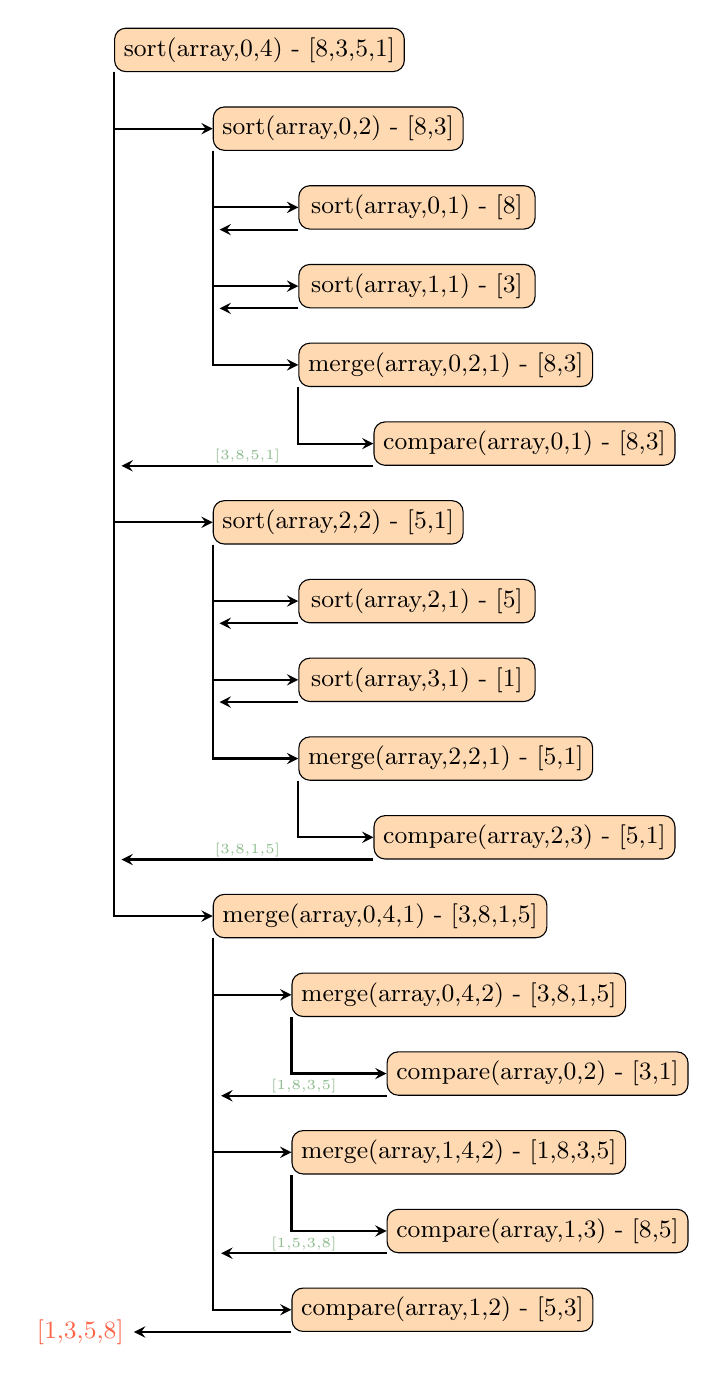
\begin{tikzpicture}[node distance=1cm, font=\small]
    \node (1) [box] {sort(array,0,4) - [8,3,5,1]};

    \node (2) [box, below of=1, xshift=1cm] {sort(array,0,2) - [8,3]};

    \node (3) [box, below of=2, xshift=1cm] {sort(array,0,1) - [8]};
    
    \node (4) [box, below of=3, xshift=0cm] {sort(array,1,1) - [3]};
    
    \node (5) [box, below of=4, anchor=west] at (4.west) {merge(array,0,2,1) - [8,3]};
    \node (6) [box, below of=5, xshift=1cm] {compare(array,0,1) - [8,3]};
    \node (7) [box, anchor=west] at ($(2.west) + (0,-5)$) {sort(array,2,2) - [5,1]};
    \node (8) [box, below of=7, xshift=1cm] {sort(array,2,1) - [5]};
    \node (9) [box, below of=8, xshift=0cm] {sort(array,3,1) - [1]};
    \node (10) [box, below of=9, anchor=west] at (9.west) {merge(array,2,2,1) - [5,1]};
    \node (11) [box, below of=10, xshift=1cm] {compare(array,2,3) - [5,1]};
    \node (12) [box, anchor=west] at ($(7.west) + (0,-5)$) {merge(array,0,4,1) - [3,8,1,5]};
    \node (13) [box, below of=12, xshift=1cm] {merge(array,0,4,2) - [3,8,1,5]};
    \node (14) [box, below of=13, xshift=1cm] {compare(array,0,2) - [3,1]};
    \node (15) [box, anchor=west] at ($(13.west) + (0,-2)$) {merge(array,1,4,2) - [1,8,3,5]};
    \node (16) [box, below of=15, xshift=1cm] {compare(array,1,3) - [8,5]};
    \node (17) [box, anchor=west] at ($(15.west) + (0,-2)$) {compare(array,1,2) - [5,3]};


    \draw [arrow] (1.south west) |- (2);
    \draw [arrow] (2.south west) |- (3);
    \draw [arrow] (2.south west) |- (4);
    \draw [arrow] (2.south west) |- (5);
    \draw [arrow] (5.south west) |- (6);
    \draw [arrow] (1.south west) |- (7);
    \draw [arrow] (7.south west) |- (8);
    \draw [arrow] (7.south west) |- (9);
    \draw [arrow] (7.south west) |- (10);
    \draw [arrow] (10.south west) |- (11);
    \draw [arrow] (1.south west) |- (12);
    \draw [arrow] (12.south west) |- (13);
    \draw [arrow] (13.south west) |- (14);
    \draw [arrow] (12.south west) |- (15);
    \draw [arrow] (15.south west) |- (16);
    \draw [arrow] (12.south west) |- (17);
    \draw [arrow] (3.south west) |- ++(-1,0);
    \draw [arrow] (4.south west) |- ++(-1,0);
    \draw [arrow] (6.south west) |- node[pos=0.75, above, yshift=-0.1cm] {\tiny{\color{DarkSeaGreen}{[3,8,5,1]}}} ++(-3.2,0);
    \draw [arrow] (8.south west) |- ++(-1,0);
    \draw [arrow] (9.south west) |- ++(-1,0);
    \draw [arrow] (11.south west) |- node[pos=0.75, above, yshift=-0.1cm] {\tiny{\color{DarkSeaGreen}{[3,8,1,5]}}} ++(-3.2,0);
    \draw [arrow] (14.south west) |- node[pos=0.75, above, yshift=-0.1cm] {\tiny{\color{DarkSeaGreen}{[1,8,3,5]}}} ++(-2.1,0);
    \draw [arrow] (16.south west) |- node[pos=0.75, above, yshift=-0.1cm] {\tiny{\color{DarkSeaGreen}{[1,5,3,8]}}} ++(-2.1,0);
    \draw [arrow] (17.south west) |- node[left, xshift=-2cm] {\color{Tomato}{[1,3,5,8]}} ++(-2,0);
  \end{tikzpicture}
  \caption{Call stack}
  \label{fig:call-stack}
\end{figure}

\newpage
Egy 8 elemű tömbre egy másik vizuális reprezentáció \cite{mit-batcher} a \ref{fig:mit-batcher}. ábrán látható.

\begin{figure}[hb]
  \centering
  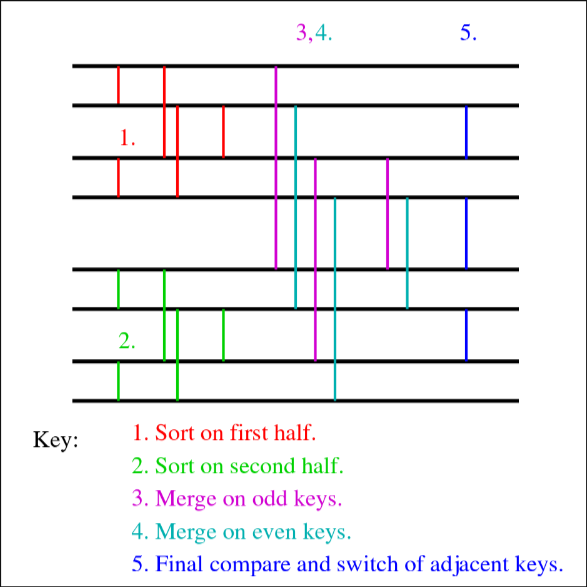
\includegraphics[width=0.8\textwidth]{mit-batcher.png}
  \caption{Batcher reprezentálás 8 inputra}
  \label{fig:mit-batcher}
\end{figure}

\section{5x5-ös medián szűrő megvalósítás}
A megvalósításhoz minden sorban komponensenként lépkedve elmentek egy 5x5-ös ablakot, erre futtatom az algoritmust, és az így rendezett tömbnek a 12-ik (medián) elemét adom vissza részeredményként.
Mielőtt átadom a rendező függvénynek a tömböt kibővítem 255-ös értékekkel (8 bites komponensek) 25-ről 32 elemre, mivel csak 2 hatvány nagyságú tömbökre működik az algoritmus.  

\newpage

\begin{lstlisting}[style=cstyle, caption={5x5 medián szűrő C-kód}, label={lst:median}]
#include "batcher.h"
#include <stdio.h>
#include "stdbool.h"
#include <cstring>

void compare(uint8_t* array, int i, int j)
{
  if (array[i]>array[j])
  {
    uint8_t tmp = array[i];
    array[i] = array[j];
    array[j] = tmp;
  }

}

void merge(uint8_t* array, int start, int length, int r)
{
  int m=r*2;
  if(m<length)
  {
    merge(array, start, length, m);
    merge(array, start+r, length, m);
    for (int i=start+r; i+r<start+length; i+=m)
      compare(array, i, i+r);
  }
  else
    compare(array, start, start+r);
}

void sort(uint8_t* array, int start, int length)
{

  if(length>1)
  {
    int m = length/2;
    sort(array, start, m);
    sort(array, start+m, m); 
    merge(array, start, length, 1);
  }

}

void media_filter_scalar(int imgHeight, int imgWidth, int imgWidthF,
			   uint8_t *imgSrcExt, uint8_t *imgDst)
{
  for(int row=0; row<imgHeight; row++)
  {
    for(int col=0; col<imgWidthF; col++)
    {
      uint8_t r_vals[25], g_vals[25], b_vals[25];
			int rd_offset;

      for(int fy=0; fy<5; fy++)
      {
        for(int fx=0; fx<5; fx++)
        {
          rd_offset = ((row+fy)*imgWidthF + (col+fx))*3;
          int idx = fy*5+fx;

          r_vals[idx] = *(imgSrcExt + rd_offset + 0);
          g_vals[idx] = *(imgSrcExt + rd_offset + 1);
          b_vals[idx] = *(imgSrcExt + rd_offset + 2);
        }
      }
      uint8_t padded_r[32], padded_g[32], padded_b[32];
      memcpy(padded_r, r_vals, 25);
      memset(padded_r + 25, 255, 7);
      memcpy(padded_g, g_vals, 25);
      memset(padded_g + 25, 255, 7);
      memcpy(padded_b, b_vals, 25);
      memset(padded_b + 25, 255, 7);

      sort(padded_r,0,32);
      sort(padded_g,0,32);
      sort(padded_b,0,32);

			int wr_offset;
			wr_offset = row*imgWidth*3 + col*3;
      
      *(imgDst + wr_offset + 0) = padded_r[12];
      *(imgDst + wr_offset + 1) = padded_g[12];
      *(imgDst + wr_offset + 2) = padded_b[12];

    }
  }
}


\end{lstlisting}
\newpage
A működést teszteltem is egy egyszerű python scripttel, ugyanazt az eredményt adja mint a referencia.

\begin{lstlisting}[style=pythonstyle, caption={Python összehasonlító}, label={lst:python-test}]
from PIL import Image, ImageChops
import sys, getopt
import numpy as np

if len(sys.argv) != 3:
    print("Usage: python test.py image1.png image2.png")
    sys.exit(1)

img1 = Image.open(sys.argv[1])
img2 = Image.open(sys.argv[2])

diff = ImageChops.difference(img1, img2)

diff_array = np.array(diff)

different_pixels = np.count_nonzero(diff_array.any(axis=2))

print(f"Differing pixels: {different_pixels}")
total_pixels = diff_array.shape[0] * diff_array.shape[1]
print(f"Total pixels: {total_pixels}")
print(f"Percentage different: {different_pixels / total_pixels * 100:.2f}%")
\end{lstlisting}


\printbibliography

\end{document}
